\documentclass[../../FisicaTeorica.tex]{subfiles}
\begin{document}

\begin{comment}
\section{Lezione X:\\ \large{Teorema delle perturbazioni indipendenti dal tempo}}
\vspace{-1em}
\begin{center}
    \small{(14/12/2018)}
\end{center}
\end{comment}

\section{Teoria delle perturbazioni}
Spesso, in \MQ, ci si trova di fronte a problemi che non sono risolvibili analiticamente, ma \q{che non si discostano eccessivamente} da altri problemi che invece lo sono. Uno strumento utile per gestire tali situazioni è dato dalla \textit{teoria perturbativa}, di cui ci occuperemo in questa sezione, limitatamente al caso di perturbazioni \textbf{indipendenti dal tempo}\marginpar{Perturbazioni indipendenti dal tempo}.\\

L'idea di fondo sta nell'esaminare come cambiano gli autostati di una hamiltoniana data dalla somma di due termini: uno che si sa risolvere in modo esatto, e un altro, più piccolo del primo, che \q{lo perturba}. Un esempio è l'atomo di idrogeno inserito in un campo magnetico debole.\\

Matematicamente, consideriamo un'Hamiltoniana $H$ scomponibile in due termini:
\begin{align}
H = H_0 + \lambda V
\label{eqn:hamiltoniana_perturbata}
\end{align}
dove di $H_0$ sappiamo autovalori e autostati, e $\lambda$ è un parametro \q{piccolo} rispetto agli altri.\\
Denotiamo gli autovalori di $H_0$ con $\mathcal{E}^0_n$, che assumeremo inizialmente \textbf{ortonormali} e\marginpar{Caso 1: Autovalori $\mathcal{E}_n^0$ non degeneri} \textbf{non degeneri}, e i rispettivi autostati con $\ket{\mathcal{E}^0_n}$. Per $H_0$ valgono allora le equazioni agli autovalori:
\begin{align*}
H_0 \ket{\mathcal{E}^0_n} = \mathcal{E}^0_n \ket{\mathcal{E}^0_n}
\end{align*}
Denotiamo invece con $\ket{\mathcal{E}_n}$ gli autostati dell'hamiltoniana $H$ \q{completa}, per cui:
\begin{align*}
H\ket{\mathcal{E}_n} = \mathcal{E}_n \ket{\mathcal{E}_n}
\end{align*}
Al limite di una perturbazione \q{nulla}, questi ultimi autovalori $\mathcal{E}_n$ tendono a quelli $\mathcal{E}_n^0$ conosciuti:\begin{align*}
\lim_{\lambda \to 0} \mathcal{E}_n = \mathcal{E}^0_n
\end{align*}

Supponiamo (\textbf{ipotesi perturbativa})\index{Ipotesi perturbativa}\marginpar{Ipotesi perturbativa} di poter espandere sia $\ket{\mathcal{E}_n}$ che $\mathcal{E}_n$ in una serie di Mac-Laurin in $\lambda$:
\begin{align}
\ket{\mathcal{E}_n} &= \ket{\mathcal{E}^0_n} + \lambda \ket{\mathcal{E}^1_n} + \lambda^2 \ket{\mathcal{E}^2_n} + \dots \label{eqn:serie_vector}\\
\mathcal{E}_n &= \mathcal{E}^0_n + \lambda \mathcal{E}^1_n + \lambda^2 \mathcal{E}^2_n +\dots \label{eqn:serie_evalue}\\
\nonumber
\mathcal{E}_n^k =\frac{1}{k!} \frac{d^k \mathcal{E}_n}{d\lambda^k}\Big|_{\lambda=0}\span \qquad \ket{\mathcal{E}_n^k}=\frac{1}{k!}\frac{d^k\ket{\mathcal{E}_n^k}}{d\lambda^k}\Big|_{\lambda=0}
\end{align}

Assumiamo come normalizzazione per gli autovettori $\ket{\mathcal{E}_n}$ la seguente espressione:
\begin{align}
\braket{\mathcal{E}^0_n|\mathcal{E}_n} \overset{!}{=} 1
\label{eqn:normalizzazione-perturbativa}
\end{align} 
Espandendo $\ket{\mathcal{E}_n}$ nella normalizzazione (\ref{eqn:normalizzazione-perturbativa}) tramite la serie di potenze in (\ref{eqn:serie_vector}) otteniamo:
\begin{align*}
1 \underset{(\ref{eqn:normalizzazione-perturbativa})} =
\braket{\mathcal{E}^0_n | \mathcal{E}_n} = 
\underbrace{\braket{\mathcal{E}_n^0|\mathcal{E}_n^0}}_{=1}
+ \lambda \braket{\mathcal{E}^0_n | \mathcal{E}^1_n} + \lambda^2 \braket{\mathcal{E}_n^0|\mathcal{E}^2_n} + \dots \quad \forall \lambda
\end{align*}
Poiché tale espressione deve valere per ogni scelta di $\lambda$, si che i coefficienti dei termini dello stesso ordine devono essere uguali. Ma poiché il membro a sinistra non contiene potenze di $\lambda$ (se non quella di ordine $0$, ricaviamo che:
\begin{align*}
\braket{\mathcal{E}_n^0|\mathcal{E}_n^k} = 0 \quad k=1,2,3,\dots
\end{align*}

\textbf{Nota}: la normalizzazione appena adottata è \textit{non canonica}, nel senso che così facendo in genere $\braket{\mathcal{E}_n|\mathcal{E}_n}\neq1$. Come vedremo nei conti seguenti, tuttavia, si dimostra una scelta utile al nostro scopo.\\ 

Per trovare gli autovalori $\mathcal{E}_n^k$ dell'espansione perturbativa partiamo dall'equazione agli autovalori generale:
\begin{align*}
(H_0+\lambda V) \ket{\mathcal{E}_n} = \mathcal{E}_n \ket{\mathcal{E}_n}
\end{align*}
Inserendo gli sviluppi in potenze (\ref{eqn:serie_vector}) e (\ref{eqn:serie_evalue}):
\begin{align} \label{eqn:autoval_espansa}
(H_0 + \lambda V) \sum_{k=0}^{\infty} \lambda^k \ket{\mathcal{E}_n^k} &= \left(\sum_{l=0}^\infty \lambda^l\mathcal{E}^l_n \right) \left( \sum_{m=0}^\infty \lambda^m \ket{\mathcal{E}^m_n}\right)\\
\nonumber
(H_0 + \lambda V)(\ket{\mathcal{E}_n^0} + \lambda\ket{\mathcal{E}_n^1}+\lambda^2\ket{\mathcal{E}_n^2}+\dots
) &=(\mathcal{E}_n^0 + \lambda \mathcal{E}_n^1 + \lambda^2\mathcal{E}_n^2+\dots)\cdot\\
&\>\>\,\cdot (\ket{\mathcal{E}_n^0} + \lambda \ket{\mathcal{E}_n^1}+\lambda^2\ket{\mathcal{E}_n^2}+\dots)
\end{align}
Nuovamente, l'espressione vale $\forall \lambda$, e quindi i coefficienti di termini dello stesso ordine devono essere uguali.

\begin{itemize}
\item All'ordine $k=0$, riotteniamo l'equazione agli autovalori per $H_0$:
\begin{align*}
H_0 \ket{\mathcal{E}_n^0} = \mathcal{E}_n^0 \ket{\mathcal{E}_n^0}
\end{align*}
\item All'ordine $k=1$, si ha invece:
\begin{align*}
H_0 \ket{\mathcal{E}^1_n} + V \ket{\mathcal{E}^0_n} = \mathcal{E}^0_n \ket{\mathcal{E}^1_n} + \mathcal{E}^1_n
 \ket{\mathcal{E}^0_n}\end{align*}
Prendendo il prodotto scalare con $\ket{\mathcal{E}_n^0}$ otteniamo:
\begin{align*}
\underbrace{\bra{\mathcal{E}^0_n} H_0 \ket{\mathcal{E}^1_n}}_{\mathcal{E}_n^0 \braket{\mathcal{E}^0_n|\mathcal{E}^1_n}=0} + \bra{\mathcal{E}^0_n}V \ket{\mathcal{E}^0_n} = \mathcal{E}_n^0\underbrace{ \braket{\mathcal{E}^0_n | \mathcal{E}^1_n}}_{=0} + \mathcal{E}^1_n
\end{align*}
Notando che $\bra{\mathcal{E}_n^0}H=\mathcal{E}_n^0\bra{\mathcal{E}_n^0}$ (per la versione duale dell'equazione di Schr\"odinger) e che $\braket{\mathcal{E}_n^0|\mathcal{E}_n^1}=0$ per la normalizzazione adottata, giungiamo a:
\begin{align*}
\mathcal{E}_n^1 = \bra{\mathcal{E}_n^0} V \ket{\mathcal{E}^0_n}
\end{align*}
E perciò $\mathcal{E}_n$, al primo ordine in $\lambda$ è dato da:
\begin{align*}
\mathcal{E}_n \approx \mathcal{E}_n^0 + \lambda \mathcal{E}_n^1 = \bra{\mathcal{E}_n^0}H_0\ket{\mathcal{E}_n^0}
+ \lambda \bra{\mathcal{E}^0_n}V\ket{\mathcal{E}^0_n} \underset{(\ref{eqn:hamiltoniana_perturbata})}{=} \bra{\mathcal{E}^0_n}H \ket{\mathcal{E}^0_n}
\end{align*}
Perciò, al I ordine in $\lambda$ l'autovalore $\mathcal{E}_n$ è il valor medio di $H$ nello stato imperturbato $\ket{\mathcal{E}^0_n}$.\\

\end{itemize}


Più in generale, all'ordine $k$:
\begin{align}
H_0 \ket{\mathcal{E}^k_n} + V\ket{\mathcal{E}^{k-1}_n} = \sum_{l=0}^k \mathcal{E}^l_n \ket{\mathcal{E}^{k-l}_n}
\label{eqn:termine-l}
\end{align}
Prendendo nuovamente il prodotto scalare con $\ket{\mathcal{E}^0_n}$: \marginpar{Espressione per $\mathcal{E}_n^k$}
\begin{align}
\underbrace{\bra{\mathcal{E}^0_n} H_0 \ket{\mathcal{E}^k_n}}_{\mathcal{E}_n^0 \braket{\mathcal{E}_n^0 | \mathcal{E}^k_n} =0} + 
\bra{\mathcal{E}^{0}_n}V\ket{\mathcal{E}^{k-1}_n} = \mathcal{E}^k_n \Rightarrow \bm{\mathcal{E}_n^k = \bra{\mathcal{E}_n^0}V\ket{\mathcal{E}_n^{k-1}}}\quad k>0
\label{enk_val_final}
\end{align}
dato che al secondo membro \textit{sopravvive} solo il termine con $k-l=0\Rightarrow l=k$, dato che i prodotti $\braket{\mathcal{E}_n^0|\mathcal{E}_n^{k-l}} = \delta_{0,k-l}$ per la normalizzazione adottata.\\

Notiamo che otteniamo una \textit{formula chiusa}. Riscrivendo il membro a sinistra di (\ref{eqn:autoval_espansa}) e prendendo il prodotto scalare con $\ket{\mathcal{E}_n^0}$:
\begin{align*}
\bra{\mathcal{E}^0_n}(H_0 + \lambda V) \left( \sum_{l=0}^\infty \lambda^l \ket{\mathcal{E}^l_n} \right) &= \bra{\mathcal{E}_n^0}H_0\ket{\mathcal{E}_n^0} + \lambda \bra{\mathcal{E}_n^0} V \ket{\mathcal{E}^0_n} + \sum_{l=1}^\infty \lambda^{l+1} \bra{\mathcal{E}_n^0}V \ket{\mathcal{E}_n^l} =\\
&\underset{(a)}{=}\mathcal{E}^0_n + \lambda \mathcal{E}^1_n + \sum_{l=1}^\infty \lambda^{l+1} \mathcal{E}^{l+1}_n = \mathcal{E}_n
\end{align*}
dove in (a) abbiamo usato le relazioni appena trovate, notando che $\bra{\mathcal{E}_n^0}H\ket{\mathcal{E}_n^0}=\bra{\mathcal{E}_n^0}H_0\ket{\mathcal{E}_n^0}=\mathcal{E}_n^0$ e, per $l\geq 1$ $\bra{\mathcal{E}_n^0}V\ket{\mathcal{E}_n^l}=\mathcal{E}_n^l$. Ritroviamo perciò, nel membro a destra, l'espansione in serie di potenze di $\mathcal{E}_n$.\\
Ricordando poi che:
\begin{align*}
\sum_{l=0}^\infty \lambda^l \ket{\mathcal{E}^l_n} =\ \ket{\mathcal{E}_n}
\end{align*}
Da cui:
\begin{align*}
\bra{\mathcal{E}_n^0}H\hlc{Yellow}{\ket{\mathcal{E}_n}} = \mathcal{E}_n^0 + \lambda\mathcal{E}_n^1 + \sum_{l=1}^\infty \lambda^{l+1}\mathcal{E}_n^{l+1}=\mathcal{E}_n
\end{align*}


Cerchiamo\marginpar{Ricerca degli autovettori $\ket{\mathcal{E}_n^k}$} ora un'espressione per i vettori $\ket{\mathcal{E}^k_n}$. Un'idea è determinarli nella base degli autovettori $\ket{\mathcal{E}^0_m}$ che conosciamo. Matematicamente, partiamo usando la completezza di Dirac per la base $\{\ket{\mathcal{E}^0_m}\}_{m\in \bb{N}}$, nell'ipotesi di \textbf{autovalori non degeneri}, da cui otteniamo l'espansione di un generico $\ket{\mathcal{E}_n^k}$:
\begin{align*}
\ket{\mathcal{E}_n^k} = \bb{I} \ket{\mathcal{E}^k_n} = \sum_{m} \ket{\mathcal{E}^0_m} \braket{\mathcal{E}^0_m|\mathcal{E}^k_n} \qquad k>0
\end{align*}
Notiamo che $\braket{\mathcal{E}^0_m|\mathcal{E}^k_n}$ è nullo se $m=n$ (per la normalizzazione introdotta). Riscriviamo quindi la somma come:
\begin{align*}
\ket{\mathcal{E}_n^k} = \sum_{m\neq n} \ket{\mathcal{E}^0_m} \braket{\mathcal{E}_m^0| \mathcal{E}^k_n}
\end{align*}

Prendendo ora il prodotto scalare con $\ket{\mathcal{E}_m^0}$ dell'equazione agli autovalori di ordine $k$ (\ref{eqn:termine-l}):
\begin{align*}
\hlc{SkyBlue}{{\bra{\mathcal{E}^0_m} H_0 \ket{\mathcal{E}^k_n}} }+ \bra{\mathcal{E}^0_m} V \ket{\mathcal{E}^{k-1}_n}
&\underset{(\ref{eqn:termine-l})}{=} \sum_{l=0}^k \mathcal{E}_n^l \braket{\mathcal{E}_m^0 | \mathcal{E}^{k-l}_n}\\
\hlc{SkyBlue}{\mathcal{E}_m^0\braket{\mathcal{E}_m^0|\mathcal{E}_n^k}} + \bra{\mathcal{E}_m^0}V\ket{\mathcal{E}_n^{k-1}}
&=\mathcal{E}_n^0 \braket{\mathcal{E}_m^0|\mathcal{E}_n^k} + \sum_{l=1}^{k}\mathcal{E}_n^l \braket{\mathcal{E}_m^0|\mathcal{E}_n^{k-l}}
\end{align*}
Isolando $\braket{\mathcal{E}_m^0 | \mathcal{E}^k_n}$:
\begin{align*}
\braket{\mathcal{E}^0_m | \mathcal{E}^k_n} = 
\frac{1}{\mathcal{E}^0_n - \mathcal{E}^0_m} \left(
\bra{\mathcal{E}^0_m}V \ket{\mathcal{E}_n^{k-1}} - \sum_{l=1}^{k} \mathcal{E}_n^l \braket{\mathcal{E}^0_m| \mathcal{E}_n^{k-l}}\right)
\end{align*}
E, sostituendo nella completezza:
\begin{align}
\ket{\mathcal{E}_n^k} = \sum_{m\neq n}\frac{\ket{\mathcal{E}_m^0}}{\mathcal{E}_n^0-\mathcal{E}_m^0} \left( \bra{\mathcal{E}_m^0}V\ket{\mathcal{E}_n^{k-1}}-\sum_{l=1}^k \mathcal{E}_n^l \braket{\mathcal{E}_m^0|\mathcal{E}_n^{k-l}}\right)
\label{eqn:Enk_final}
\end{align}
L'espressione è ben definita dato che, per ipotesi di nondegenerazione, $\mathcal{E}_n^0 \neq \mathcal{E}_m^0$ per $m\neq n$ (e per $m=n$ $\braket{\mathcal{E}_m^0|\mathcal{E}_m^k}=\delta_{0,k}$ dalla normalizzazione).\\
Notiamo ora che il termine di destra contiene solo termini \q{precedenti} nell'espansione, del tipo $\ket{\mathcal{E}_n^s}$ con $s < k$. Anche gli autovalori $\mathcal{E}_n^l$ che compaiono richiedono, per essere calcolati, termini \textit{precedenti}, data la formula trovata in (\ref{enk_val_final}):
\begin{align*}
\mathcal{E}_n^k = \bra{\mathcal{E}_n^0}V\ket{\mathcal{E}^{k-1}_n}
\end{align*}
Perciò possiamo procedere \textit{iterativamente}, calcolando $\ket{\mathcal{E}_n^{k+1}}$ a partire dai $\ket{\mathcal{E}_n^k}$ di ordine inferiore già determinati, e così ricavare tutta l'espansione.\\

Sostituendo le espressioni per $\ket{\mathcal{E}_n^k}$ nell'espansione per $\ket{\mathcal{E}_n}$ in (\ref{eqn:serie_vector}) giungiamo a:
\marginpar{Formula per gli autovettori $\ket{\mathcal{E}_n}$}
\begin{align*}
\ket{\mathcal{E}_n} = \ket{\mathcal{E}_n^0} + \lambda \sum_{m\neq n} \ket{\mathcal{E}^0_m} \frac{\overbrace{\bra{\mathcal{E}^0_m}V \ket{\mathcal{E}^0_n}}^{\braket{\mathcal{E}_m^0|\mathcal{E}^1_n}}}{\mathcal{E}_n^0 - \mathcal{E}_m^0} + \dots
\end{align*}
\begin{enumerate}
\item Il primo termine:
\begin{align} \nonumber
\mathcal{E}_n^1 &= \bra{\mathcal{E}^0_n}V \ket{\mathcal{E}^0_n}\\
\ket{\mathcal{E}_n^1} &\underset{(\ref{eqn:Enk_final})}{=} \sum_{m\neq n} \ket{\mathcal{E}^0_m} \frac{\bra{\mathcal{E}^0_m}V\ket{\mathcal{E}^0_n}-\bcancel{\mathcal{E}_n^1 \braket{\mathcal{E}_m^0|\mathcal{E}_n^0}}}{\mathcal{E}^0_m - \mathcal{E}^0_n} =
\sum_{m\neq n}\ket{\mathcal{E}_m^0}\frac{\bra{\mathcal{E}_m^0}V\ket{\mathcal{E}_n^0}}{\mathcal{E}_m^0-\mathcal{E}_n^0}
\label{eqn:En1-vec}
\end{align}
\item Per il secondo termine, invece, otteniamo:
\begin{align*}
\mathcal{E}_n^2 &\underset{(\ref{enk_val_final})}{=} \bra{\mathcal{E}_n^0}V \ket{\mathcal{E}_n^1} = \sum_{m\neq n} \frac{\bra{\mathcal{E}_n^0}V\ket{\mathcal{E}_m^0} \bra{\mathcal{E}_m^0}V\ket{\mathcal{E}_n^0}}{\mathcal{E}_n^0 - \mathcal{E}_m^0} = \sum_{m\neq n} \frac{|\bra{\mathcal{E}_n^0}V \ket{\mathcal{E}_n^0}|^2}{\mathcal{E}_n^0 - \mathcal{E}^0_m}
\end{align*}
\end{enumerate}

Finora abbiamo utilizzato una normalizzazione \textit{non canonica}, per cui $\braket{\mathcal{E}_n|\mathcal{E}_n^0} = 1$. Se vogliamo passare alla normalizzazione \q{usuale} è perciò necessario un passaggio di \textit{rinormalizzazione}. \marginpar{Normalizzazione canonica}
Denotando il risultato con $\ket{\mathcal{E}_n}^N$, tale che $\prescript{N}{}{\braket{\mathcal{E}_n|\mathcal{E}_n}}^N = 1$, otteniamo:
\begin{align*}
\ket{\mathcal{E}_n}^N = z^\frac{1}{2} \ket{\mathcal{E}_n} \quad \braket{\mathcal{E}_n| \mathcal{E}_n^0} = 1
\end{align*}
$z$ è detta \textit{costante di rinormalizzazione} della funzione d'onda.\\
Si trova $z=1$ per il primo ordine, mentre per $k=2$:
\begin{align*}
\lambda^2 \Rightarrow  z_2 = 1-\lambda^2 \sum_{m\neq n} \frac{|\bra{\mathcal{E}_m^0}V\ket{\mathcal{E}^0_n}|^2}{(\mathcal{E}_n^0 - \mathcal{E}_m^0)^2}
\end{align*}
Possiamo ora calcolare agilmente le probabilità di misura.
Se il sistema è in un autostato $\ket{\mathcal{E}_n}$ di $H$, la probabilità che una misura la trovi nello stato $\ket{\mathcal{E}^0_n}$ è:
\begin{align*}
p = \left| \prescript{N}{}{\braket{\mathcal{E}_n | \mathcal{E}_n^0 }} \right|^2
\end{align*}
Dove la $N$ ad apice a sinistra indica che stiamo usando il \textit{bra} normalizzato canonicamente, duale di $\ket{\mathcal{E}_n}^N$.\\

Cosa succede se rimuoviamo l'ipotesi che\marginpar{Caso 2: Autovalori $\mathcal{E}_n^0$ degeneri} $H_0$ abbia solo autovalori nondegeneri?\\
Supponiamo che $\mathcal{E}^0_n$ sia \textit{degenere} e che $\{\ket{\mathcal{E}^0_{n}, i} \text{ autoket con } i = 1, \dots, d(n) = \op{deg}(\mathcal{E}_n^0) \}$ sia una base dell'autospazio $\hs_n$ corrispondente all'autovalore $\mathcal{E}_n^0$ di $H_0$.\\
Nei calcoli precedenti era cruciale che $\mathcal{E}_n^0 \neq \mathcal{E}^0_m$, per evitare l'annullarsi del denominatore. In presenza di degenerazione, tuttavia, ciò accade.\\
Infatti, se sostituiamo alla completezza di Dirac la sua versione \textit{con degenerazione}:
\begin{align*}
\bb{I}=\sum_m \ket{\mathcal{E}_m^0} \bra{\mathcal{E}^0_m} \to \bb{I} = \sum_m \sum_{i=1}^{d(m)} \ket{\mathcal{E}^0_m, i} \bra{\mathcal{E}^0_m, i}
\end{align*}
ripetendo i passaggi di prima, giungiamo all'espressione:
\begin{align*}
\mathcal{E}_m^0 \braket{\mathcal{E}_m^0,i|\mathcal{E}_n^k} + \bra{\mathcal{E}_m^0,i}V \ket{\mathcal{E}_m^{k-1}} = \mathcal{E}_n^0 \braket{\mathcal{E}_m^0,i|\mathcal{E}_n^k} + \sum_{l=1}^k\mathcal{E}_n^l \braket{\mathcal{E}_m^0|\mathcal{E}_n^{k-l}}
\end{align*}
da cui non possiamo più ricavare $\braket{\mathcal{E}_m^0,i|\mathcal{E}_n^k}$, dato che dovremmo dividere per $\mathcal{E}_n^0-\mathcal{E}_m^0$ che non sempre è $\neq 0$.\\


Per eliminare questi problemi osserviamo che $1/(\mathcal{E}_n^0-\mathcal{E}^0_m)$ compare, per esempio in (\ref{eqn:En1-vec}), moltiplicato per un fattore che, nel caso con degenerazione, è del tipo $\bra{\mathcal{E}^0_n,\alpha}V\ket{\mathcal{E}^0_m,\beta}$.\\
Poiché abbiamo libertà nella scelta degli autovettori generalizzati (basta che siano una qualsiasi base dell'autospazio dell'autovalore esaminato), possiamo sceglierli in modo che gli elementi di matrice:
\begin{align*}
\bra{\mathcal{E}^0_n,\alpha}V \ket{\mathcal{E}^0_m, \beta} = 0 \Leftrightarrow \alpha \neq \beta
\end{align*}
Perciò, scegliendo così i ket $\{\ket{\mathcal{E}_n^0, \alpha}\}$ come una base dell'autospazio $\hs_n$ di autovalore $\mathcal{E}_n^0$ in cui $V$ è diagonale, il problema precedente si risolve perché ogni termine $1/(\mathcal{E}^0_n - \mathcal{E}^0_n)$ che divergerebbe ha come numeratore $\bra{\mathcal{E}^0_n, \alpha}V\ket{\mathcal{E}^0_n, \beta} = 0$ per $\beta \neq \alpha$.\\
Perciò gli stessi argomenti del caso non degenere si applicano al caso degenere con questa scelta di base, che è possibile se $V$ è \textbf{simmetrico}. Perciò, riadattando le formule precedentemente ricavate:
\begin{align}
\mathcal{E}_n^\alpha &= \mathcal{E}_n^0 + \lambda \bra{\mathcal{E}_{n}^0, \alpha}V \ket{\mathcal{E}_n^0, \alpha} + \lambda^2 \sum_{m\neq n} \sum_\beta^{d(m)} \frac{|\bra{\mathcal{E}_m^0, \beta}V \ket{\mathcal{E}^0_n,\alpha}|^2}{\mathcal{E}_n^0-\mathcal{E}^0_m} + \dots 
\label{eqn:autoval_non_deg}
\\
\ket{\mathcal{E}_n,\alpha} &= \ket{\mathcal{E}_n^0,\alpha} + \lambda \sum_{m\neq n} \sum_{\beta}^{d(n)} \ket{\mathcal{E}^0_m,\alpha} \frac{{\bra{\mathcal{E}^0_m,\alpha}V \ket{\mathcal{E}^0_n,\beta}}}{\mathcal{E}_n^0 - \mathcal{E}_m^0} + \dots
\end{align}
Con una scelta delle basi $\ket{\mathcal{E}_n,\alpha}$ tale che:
\begin{align*}
\bra{\mathcal{E}_m^0, \beta}V\ket{\mathcal{E}_n^0, \alpha}&=0 \quad m\neq n\\
\bra{\mathcal{E}_{\bm{n}}^0, \beta}V \ket{\mathcal{E}_{\bm{n}}^0,\alpha}&=0 \quad \alpha \neq \beta
\end{align*}

\subsection{Conseguenze delle perturbazioni}
In generale, se a $\mathcal{E}_n^0$ degenere sono associati $d(n)$ autovettori (di $H_0$) generalizzati $\ket{\mathcal{E}^0_n, \alpha}$, con $\alpha = 1, \dots, d(n)$, i relativi autovettori della $H$ \q{completa} $\ket{\mathcal{E}_n,\alpha}$ non saranno più degeneri, ma corrisponderanno a diversi autovalori  $\mathcal{E}_n^\alpha, \mathcal{E}_n^\beta,\dots$, come si può notare dalla formula (\ref{eqn:autoval_non_deg}).\\
 

Un'\textbf{applicazione} particolarmente interessante si ottiene partendo dall'Hamiltoniana $H_0$ dell'atomo di idrogeno, e perturbandola introducendo un campo elettrico uniforme lungo $\hat{z}$:
\begin{align*}
H = H_0 + \lambda V = H_0 + \lambda eEz
\end{align*}
dove ci interessa il caso per $\lambda = 1$.\\
Il sistema così descritto consente di analizzare il cosiddetto \textbf{effetto Stark}\footnote{Fonti utili: \url{http://bit.ly/2SsPHYD}, \url{http://bit.ly/2D5teHj}}.\index{Effetto\ Stark}\marginpar{Effetto Stark}\\

Detti $\ket{n,l,m}$ gli autostati conosciuti di $H_0$ (ignoriamo lo spin degli elettroni), concentriamoci sul caso (semplice) con $n=2$, per cui avremo $4$ orbitali degeneri, dato che (ignorando la struttura fine) l'energia dipende solo da $n$:
\begin{align*}
2s^0 && 2p^{-1} && 2p^0 && 2p^{+1}\\
\ket{2,0,0} && \ket{2,1,-1} && \ket{2,1,0} && \ket{2,1,1}
\end{align*}\\
Al primo ordine in $\lambda$, gli autovalori dell'Hamiltoniana $H$ si ottengono dalla (\ref{eqn:autoval_non_deg}):
\begin{align}
\mathcal{E}_n^\alpha = \mathcal{E}_n^0 + \lambda {\bra{\mathcal{E}_n^0, \alpha}V \ket{\mathcal{E}_n^0, \alpha}}
\label{eqn:autoval_primo_ordine}
\end{align}
dove per $\ket{\mathcal{E}_n^0,\alpha}$ dobbiamo scegliere la base in cui $V$ è diagonale, ossia tale che:
\begin{align*}
\bra{\mathcal{E}_n^0, \alpha}V\ket{\mathcal{E}_n^0,\beta} = 0 \quad \forall \alpha \neq \beta
\end{align*}
Nel caso degli autostati dell'idrogeno, tale relazione \textbf{non} è soddisfatta dalla base di autoket $\ket{n,l,m}$ da cui siamo partiti, cioè:
\begin{align*}
eE\hlc{Yellow}{\bra{n,l,m}z\ket{n,l',m'}} \neq 0 \quad \forall l\neq l', m\neq m'
\end{align*}
Infatti, calcolando gli elementi di matrice del termine evidenziato non si ottiene una matrice diagonale. Dovremo quindi diagonalizzarla e considerare la base dei suoi autovettori, e solo alla fine applicare la formula delle perturbazioni.\\
Svolgiamo allora i conti. Fissando $l$, osserviamo che:
\begin{align*}
\bra{n,l,m}z \ket{n,l,m'} = 0 \quad \forall m\neq m'
\end{align*}
Infatti gli $m$ sono gli autovalori di $L_3$, con cui $z$ commuta, dato che $L_3$ genera le rotazioni attorno a $\hat{z}$: $[z, L_3]=0$.\\
Ciò si nota esplicitamente passando in coordinate polari:
\begin{align*}
z =\ r\cos\theta; \> L_3=-i\hbar \frac{\partial}{\partial \varphi} \Rightarrow [z,L_3]=0
\end{align*}
Perciò, per $m\neq m'$ a $l$ fissato:
\begin{align*}
0 &= \bra{n,l,m} \overbrace{[z,L_3]}^{=0} \ket{n,l,m'} =\\
&= \bra{n,l,m} zL_3 \ket{n,l,m'} - \bra{n,l,m}L_3z \ket{n,l,m'}=\\
&=m' \bra{n,l,m}z \ket{n,l,m'} - m\bra{n,l,m}z \ket{n,l,m'}=\\
&= \underbrace{(m-m')}_{\neq 0} \bra{n,l,m}z \ket{n,l,m'} \Rightarrow \bra{n,l,m}z \ket{n,l,m'} = 0
\end{align*}
Notiamo poi che anche gli elementi diagonali (ossia con $m=m'$ e $l=l'$) della matrice sono nulli, poiché le autofunzioni $\ket{n,l,m}$ sono \textbf{simmetriche}: sono infatti date da polinomi di Legendre, che sono o \textit{pari} o \textit{dispari}\footnote{Ciò deriva da un fatto generale, per cui in caso di un potenziale simmetrico - come quello Coulombiano per l'idrogeno - è sempre possibile scegliere una base di autofunzioni costituita da autofunzioni simmetriche, ossia sempre o pari o dispari.}. Se calcoliamo allora $\bra{n,l,m}z\ket{n,l,m}$ in rappresentazione $\{\vec{x}\}$:
\begin{align*}
\bra{n,l,m}z\ket{n,l,m} = \int_{\bb{R}}z\psi^*(x,y,z)\psi(x,y,z)
\end{align*}
dove $\psi(x,y,z)$ è o pari o dispari. Il prodotto di due funzioni pari è pari, e anche quello di due funzioni dispari, e perciò $\psi^*\psi$ è sempre pari. Moltiplicando allora per $z$, che è dispari, si ha un'integrazione di una funzione dispari ($z\psi^*\psi$) su un dominio simmetrico rispetto all'origine, che è perciò nulla.\\
La stessa considerazione, usando solo la notazione di Dirac, si ottiene trasformando per parità l'operatore $z$, con $\mathcal{P}z\mathcal{P}=-z$. Se $\ket{n,l,m}$ è pari avremo poi $\bra{n,l,m}\mathcal{P}=+1\bra{n,l,m}$, mentre se è dispari $\bra{n,l,m}\mathcal{P}=-1\bra{n,l,m}$, con relazioni analoghe per i ket. Perciò:
\begin{align*}
\bra{n,l,m}\mathcal{P}z\mathcal{P} \ket{n,l,m} &= (\pm 1)^2 \bra{n,l,m}z \ket{n,l,m}\\
-\bra{n,l,m}z\ket{n,l,m} &= \bra{n,l,m}z\ket{n,l,m}\Rightarrow \bra{n,l,m}z\ket{n,l,m} =0
\end{align*}

Gli unici elementi di matrice non nulli, per cui $n=2$, $\hlc{Yellow}{m=m'}$ e $\hlc{SkyBlue}{l\neq l'}$ sono quindi:
\begin{align*}
\bra{2,1,0}z \ket{2,0,0}, \bra{2,0,0}z \ket{2,1,0}
\end{align*}

In forma matriciale, prendendo come base dell'autospazio $\hs_{n=2}$ (in ordine) $\{\ket{2,0,0}$, $\ket{2,1,-1}$, $\ket{2,1,0}$, $\ket{2,1,1}\}$, $\bra{n,l,m}z\ket{n,l',m'}$ è dato da:
\begin{align*}
\begin{pmatrix}
\hlc{Yellow}{\bra{2,0,0}z\ket{2,0,0}} & \hlc{SkyBlue}{\bra{2,1,-1}z\ket{2,0,0}} & \hlc{ForestGreen}{\bra{2,1,0}z\ket{2,0,0}} & \hlc{SkyBlue}{\bra{2,1,1}z\ket{2,0,0}} \\
\hlc{SkyBlue}{\bra{2,0,0}z\ket{2,1,-1}} & \hlc{Yellow}{\bra{2,1,-1}z\ket{2,1,-1}} & \hlc{SkyBlue}{\bra{2,1,0}z\ket{2,1,-1}} & \hlc{SkyBlue}{\bra{2,1,1}z\ket{2,1,-1}}\\
\hlc{ForestGreen}{\bra{2,0,0}z\ket{2,1,0}} & \hlc{SkyBlue}{\bra{2,1,-1}z\ket{2,1,0}}& \hlc{Yellow}{\bra{2,1,0}z\ket{2,1,0}} & \hlc{SkyBlue}{\bra{2,1,1}z\ket{2,1,0}}\\
\hlc{SkyBlue}{\bra{2,0,0}z\ket{2,1,1}} & \hlc{SkyBlue}{\bra{2,1,-1}z\ket{2,1,1}} &\hlc{SkyBlue}{\bra{2,1,0}z\ket{2,1,1}} & \hlc{Yellow}{\bra{2,1,1}z\ket{2,1,1}}
\end{pmatrix}
\end{align*}
Solo i termini \q{doppiamente evidenziati} (in verde) sono non nulli:
\begin{align*}
\braket{n,l,m}z\ket{n,l',m'} = \begin{pmatrix}
0 & 0 & \bra{2,1,0}z\ket{2,0,0} & 0\\
0 & 0 & 0 & 0\\
\bra{2,0,0}z\ket{2,1,0} & 0 & 0 & 0\\
0 & 0 & 0 & 0
\end{pmatrix}
\end{align*}
 
Procediamo con i conti, usando la forma esplicita per le autofunzioni $\ket{n,l,m}$ vista in (\ref{eqn:autostati_idrogeno_normalizzati}). Passando allora in rappresentazione $\{r,\theta,\varphi\}$ in $\hs=L^2(\bb{R}_+, r^2\,dr)\otimes L^2(S^2,d\Omega)$ calcoliamo il prodotto scalare $\bra{2,0,0}z\ket{2,1,0}$.\\
Gli autostati che ci interessano sono, esplicitamente:
\begin{align*}
\psi_{2,0,0}(r,\theta,\varphi)&=\frac{1}{\sqrt{8a^3}}\exp\left(-\frac{r}{2a}\right)L_1^1\left(\frac{r}{a}\right)Y_0^0(\theta,\varphi)\\
\psi_{2,1,0}(r,\theta,\varphi)&=\frac{1}{\sqrt{8a^3}}\frac{1}{\sqrt{3}}\left(\frac{r}{a}\right)\exp\left(-\frac{r}{2a}\right)L_0^3\left(\frac{r}{a}\right)Y_1^0(\theta,\varphi)
\end{align*}
con le espressioni per le armoniche sferiche e i polinomi generalizzati di Laguerre dati da:
\begin{align*}
Y_0^0(\theta,\varphi) &= \frac{1}{\sqrt{4\pi}}&& Y_1^0(\theta,\varphi) = \sqrt{\frac{3}{4\pi}}\cos\theta\\
L_0^a(x) &= 1 && L_1^a(x) = 1+a -x
\end{align*}
Con $z=r\cos\theta$ l'integrale diviene:     
\begin{align*}
\bra{2,0,0}z \ket{2,1,0} &= \int_0^{\infty}r^2\, dr \int_{0}^\pi \sin\theta\, d\theta \int_0^{2\pi}d\varphi \> \psi_{2,0,0}(r,\theta,\varphi)\,z\,\psi_{2,1,0}(r,\theta,\varphi)=\\
&=\frac{1}{32\pi a^3} \int_0^{\infty} dr\, \frac{r^4}{a}\left(2-\frac{r}{a}\right) \exp\left(-\frac{r}{a}\right) \underbrace{\int_0^\pi \cos^2(\theta)\sin(\theta) d\theta}_{2/3} \underbrace{\int_0^{2\pi} d\varphi}_{2\pi} =\\
&\underset{(a)}{=}\frac{a}{24}\int_0^{\infty}dy\, y^4 (2-y)e^{-y} =-3a
\end{align*}
dove in (a) si è effettuata la sostituzione $y = r/a$, da cui $dr = a\,dy$.\\
Si ricava poi $\bra{2,1,0}z\ket{2,0,0}=(\bra{2,0,0}z\ket{2,1,0})^*$: in questo caso i due coincidono in quanto puramente reali.\\
Reintroducendo il fattore $eE$ del potenziale, la matrice completa $\bra{n,l,m}V\ket{n,l,m}$, nella base di $\hs_{n=2}$ (in ordine) $\{\ket{2,0,0}, \ket{2,1,-1}, \ket{2,1,0}, \ket{2,1,1}\}$, diviene:
\begin{align*}
\bra{n,l,m}V\ket{n,l,m}=
\begin{pmatrix}
0 & 0 & -3aeE & 0\\
0 & 0 & 0 & 0\\
-3aeE & 0 & 0 & 0\\
0 & 0 & 0 & 0
\end{pmatrix}
\end{align*}
Per poter applicare la teoria perturbativa, è necessario passare nella base in cui $\bra{n,l,m}V\ket{n,l,m}$ è diagonale - che certamente esiste perché $V$ è simmetrico, e quindi i suoi elementi di matrice formano una matrice simmetrica e diagonalizzabile.\\
In questo caso troviamo come autovalori $0$ con molteplicità $2$, e $\lambda_\pm = \pm 3aeE$. I rispettivi autovettori, scritti in termini della base, sono dati da:
\begin{align*}
\ket{u_0,1} &= \ket{2,1,-1}; \> \ket{u_0,2}= \ket{2,1,1}; && \lambda = 0\\
\ket{u_0,3}=\ket{u_+} &= \frac{1}{\sqrt{2}}(\ket{2,0,0}-\ket{2,1,0}); && \lambda_+ = +3aeE\\
\ket{u_0,4}=\ket{u_-} &= \frac{1}{\sqrt{2}}(\ket{2,0,0}+\ket{2,1,0}; && \lambda_- = -3aeE
\end{align*}
Possiamo ora applicare la teoria perturbativa. Al primo ordine, da (\ref{eqn:autoval_primo_ordine}), ponendo $\lambda=1$:
\begin{align*}
\mathcal{E}_n^\alpha = \mathcal{E}_n^0 + \bra{\mathcal{E}_n^0,\alpha}V \ket{\mathcal{E}_n^0,\alpha}
\end{align*}
dove i $\ket{\mathcal{E}_n^0,\alpha} = \ket{u_0, \alpha}$ sono gli autovettori appena calcolati, che finalmente rispettano $\bra{\mathcal{E}_n^0,\alpha}V\ket{\mathcal{E}_n^0, \beta} = 0$ per $\alpha\neq \beta$. $\alpha$ è poi l'indice che scorre sulla degenerazione (in $H_0$) dei $\ket{\mathcal{E}_n^0, \alpha}$ di autovalore (in $H_0$) pari a $\mathcal{E}_n^0$, e che in questo caso va da $1$ a $4$. Svolgendo i conti:
\begin{align*}
\mathcal{E}_n^{\alpha=1} &= \mathcal{E}_n^{\alpha=2} = \mathcal{E}_n^0\\
\mathcal{E}_n^{\alpha=3} &= \mathcal{E}_n^0+3aeE\\
\mathcal{E}_n^{\alpha=4} &= \mathcal{E}_n^0 - 3aeE
\end{align*}

Perciò per $n=2$ si ha che gli stati che prima erano degeneri, tutti e quattro con energia $\mathcal{E}_n^0$,  \q{si splittano} e assumono tre energie diverse, come visibile in figura \ref{fig:stark_n2}.

\begin{figure}[H]
\centering
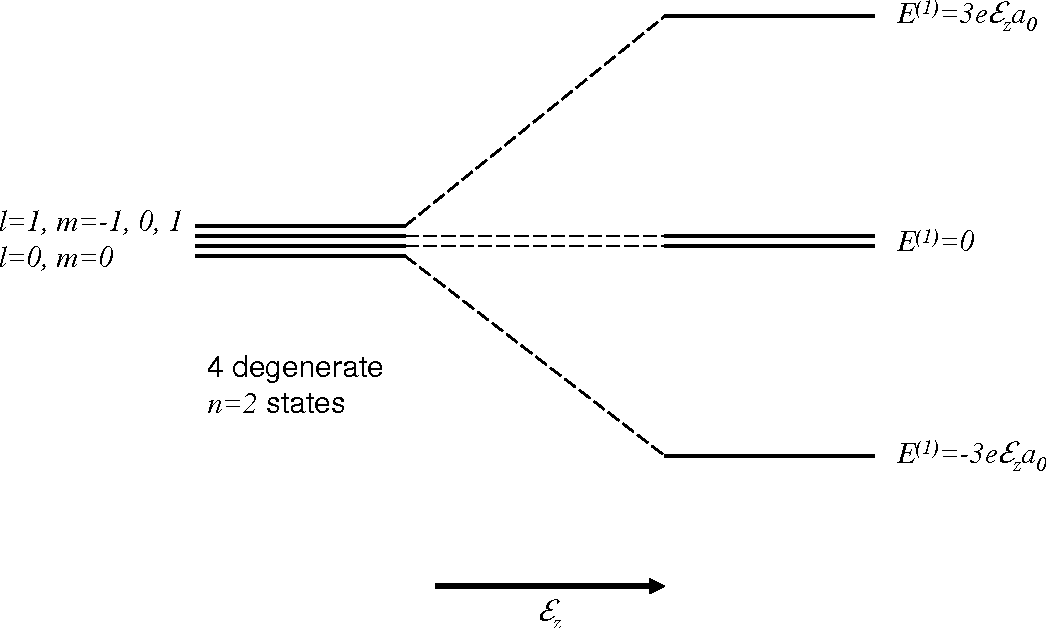
\includegraphics[scale=0.3]{Immagini/14_12/image001.png}
\caption{Effetto Stark per il livello $n=2$ dell'idrogeno: in presenza di un campo elettrico esterno, stati che prima erano degeneri non lo sono più.\label{fig:stark_n2}}
\end{figure}

Le conclusioni ottenute tramite la teoria perturbativa al primo ordine sono vicine a quanto si ottiene sperimentalmente, ma sono parziali.\\
Oppenheimer, infatti,\marginpar{L'osservazione di Oppenheimer} osservò che, sovrapponendo il potenziale elettrico con quello \textit{effettivo} coulombiano, per esempio esaminando il diagramma dell'energia in una sezione parallela all'asse $\hat{z}$ come in figura \ref{fig:tunneling_ionization},
si presenta la possibilità che un elettrone \q{di core}, ossia \textit{legato} \q{in profondità} all'atomo di idrogeno, per effetto tunnel si muova in una regione \textit{non legata}, e cioè a spettro continuo. L'esistenza di tale effetto, perciò, invaliderebbe l'esistenza stessa di stati legati per tale sistema.\\
Tale osservazione, teoricamente valida, non è predetta né dalla teoria perturbativa (anche ad ordini maggiori), né è osservata sperimentalmente. Cerchiamo di capirne il perché. 
\begin{figure}[H]
\centering
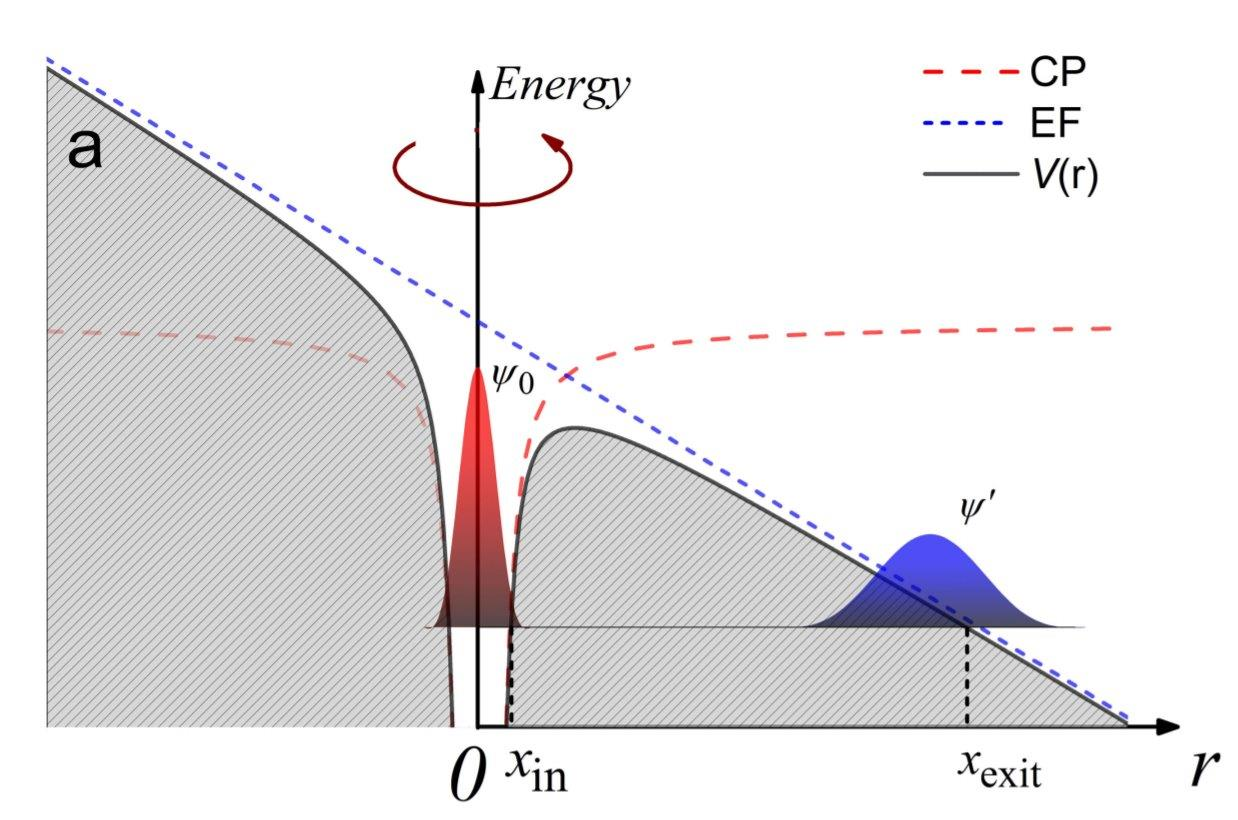
\includegraphics[scale=0.3]{Immagini/14_12/image002.jpg}
\caption{Il potenziale centrale (CP) coulombiano, sovrapposto a quello (EF) di un campo elettrico uniforme produre un $V(r)$, che, sufficientemente lontano dal nucleo, è più basso dell'energia degli elettroni negli stati \textit{legati} interni, che quindi hanno la possibilità di uscire per effetto tunnel.\label{fig:tunneling_ionization}}
\end{figure}
Per una particella di massa $m$ ed energia $\mathcal{E}$ che urta contro una barriera di potenziale $\bar{V}$ larga $L$ la probabilità di oltrepassarla per effetto tunnel è dell'ordine ricavato in (\ref{eqn:effetto_tunnel}):
\begin{align*}
\Pi \sim \exp\left(\frac{-2m\sqrt{\bar{V}-\mathcal{E}}}{\hbar}2L\right)
\end{align*}
Stimiamo l'energia di un elettrone in uno stato legato nell'atomo di idrogeno (immerso nel campo elettrico) usando l'espressione per le \textit{energie di Bohr} (\ref{eqn:bohr_energy}):
\begin{align*}
\mathcal{E}_n^0 \sim -\frac{me^4}{2\hbar^2}\frac{1}{n^2}
\end{align*}
Poiché la buca di potenziale del nucleo di idrogeno è molto stretta, per un campo elettrico sufficientemente basso è considerabile \textit{simmetrica}, per cui la sua altezza $\bar{V} \sim 0$. Otteniamo quindi la stima per $\Pi$, con $n=2$ (stato \q{profondamente legato}):
\begin{align*}
\Pi \sim \exp\left(-\frac{2L}{\hbar}\sqrt{\frac{2m^2 e^4}{4\hbar^2}}\right)= \exp\left(-L \frac{me^2}{\hbar^2}\right)=\exp\left(-\frac{L}{a}\right) \quad a = \frac{\hbar^2}{me^2}
\end{align*}
dove $a$ è il raggio di Bohr.\\
Sempre poiché la \textit{buca} del potenziale coulombiano è molto stretta, stimiamo $L$ come l'ascissa dell'intersezione tra il potenziale $y=V(x)$ e $y=-|\mathcal{E}|$ (che corrisponde a $x_{exit}$ in figura \ref{fig:tunneling_ionization}, dove consideriamo $x_{in}\approx 0$). Otteniamo allora:
\begin{align*}
-eEz  - \frac{e^2}{z} = -|\mathcal{E}| \Rightarrow  L = \frac{|\mathcal{E}| + \sqrt{|\mathcal{E}|^2 - 4e^3 E}}{2eE} \underset{E\ll1}{\sim} \frac{|\mathcal{E}|}{eE}
\end{align*}
Da cui otteniamo:
\begin{align}
\Pi \sim \exp \left(-\frac{1}{a}\frac{|\mathcal{E}|}{eE}\right)
\label{eqn:tunnel_ionization}
\end{align}
che ha una singolarità essenziale per $E=0$, e quindi non è qui espandibile in una serie di Mac-Laurin come si era supposto per applicare la teoria perturbativa. Ecco allora perché l'effetto di \textit{ionizzazione tunnel} suggerito da Oppenheimer risulta \q{invisibile} agli sviluppi perturbativi.\\\

Del resto, sperimentalmente, il fenomeno non è osservato in quanto estremamente raro per campi elettrici \q{ragionevoli}.\\
Proviamo infatti ad inserire qualche numero in (\ref{eqn:tunnel_ionization}). Prendendo l'energia dello stato fondamentale $\mathcal{E}/e=-13.6$V, $a=0.5\times 10^{11}$m e per $E = 10^5$V/m (generato per esempio in un condensatore piano con lastre distanti $1$m e con una $\Delta V=100$kV tra di esse), si ha:
\begin{align*}
\Pi \sim 10^{-6\cdot 10^6 }
\end{align*}
che è infinitamente piccolo (per confronto, le particelle nell'intero universo osservabile sono stimate attorno a $10^{75}$). Perciò, seppur matematicamente lo spettro di un atomo di idrogeno in campo elettrico sia continuo, nella pratica ne osserviamo solo uno spettro discreto - e l'effetto di \textit{ionizzazione tunnel} è rilevabile solo usando appositi apparati, con campi elettrici estremamente intensi, per cui però la teoria perturbativa è inapplicabile in partenza.

\end{document}

